\documentclass{article}

\usepackage[table]{xcolor}
\usepackage{amsmath, physics, gensymb, microtype, float, multicol}
\usepackage{tikz, tikz-3dplot, pgfplots}
\usepackage[letterpaper, bottom=1in, top=1in, left=1in, right=1in]{geometry}

\pgfplotsset{compat=newest}

\newcommand{\dt}{\mathrm{d}t}
\newcommand{\x}{\mathrm{x}}
\newcommand{\y}{\mathrm{y}}
\newcommand{\z}{\mathrm{z}}
\newcommand{\vel}{\mathrm{v}}
\newcommand{\ddt}[1]{\frac{\mathrm{d}#1}{\dt}}
\newcommand{\dydt}{\frac{\mathrm{d}y}{\dt}}

\patchcmd\subequations
 {\theparentequation\alph{equation}}
 {\subequationsformat}
 {}{}
\newcommand{\subequationsformat}{\theparentequation.\arabic{equation}}

\title{Report 1: Measurements}
\date{2/10/2023}
\author{Laith Toom}

\begin{document}
\maketitle 

\noindent Phys 207 Lab CD4

\noindent \textbf{Instructor:} Georgios Goulas

\noindent \textbf{Group:} Radjabov Jake and Tenzin Tsepak

\vspace{1em}
\hrule
\section{Introduction}
This lab is meant to explore the relationship between different variables, 
or the lack thereof.

\vspace{1em}
\hrule
\section{Procedure}

\subsection{Head Circumference and Heartbeat Time}
Each group will pick one of their members to be their test subject. First, we will measure the 
circumference of their head by using a rope and a ruler in cm. Then, we will time between 
two of their heartbeats. We will enter this data onto the computer to use at the end of the lab.

\subsection{Estimate $\pi$}
We are meant to find the circumference and diamater of various objects, then calculate 
the ratio between the two using the formula:
\[ \frac{C}{D}=\pi \]
The calculated value will only be an esimate of $\pi$, but it should be relatively close.

\subsubsection{3 Objects}
There are 3 circular objects:
\begin{enumerate}
    \item A 500-gram mass.
    \item A small circular disk.
    \item A large circular disk.
\end{enumerate}
For each object, we measure their circumference and diameter using a ruler, in which these values
will be recorded in a Microsoft Excel spreadsheet. Then, we create a scatter plot in Excel, with 
the $x$-axis representing diameter and the $y$-axis representing circumfernece. Our estimate 
of $\pi$ for this test will be the slope of the trendline of our poltted data.

\subsubsection{Toothpicks}
We form a circular shape using toothpicks. The circumference will be the amount 
of toothpicks used to form the shape and the diameter will be roughly the amount 
of toothpicks it takes to divide the shape in half. We then calculate our $\pi$ 
estimate using these measurements.

\subsubsection{Google Maps}
We will find a circular building or geographic location. Then, using the measure
distance feature of Google Maps, plot points around the circumference of the object to 
find the circumference and plot two points perpendicular to each other as well as the center of 
the object to find the diameter. We will then calculate our estimate of $\pi$ using these 
measurements.

\subsection{Calculate Uncertainty in Measurements}
We will calculate the potential uncertaintiy in different measurements.

\subsubsection{Measure the Fish}
We will measure the length of a printed image of a fish using a ruler in centimeters. Then, we will calculate
the uncertaintiy of this measurement by taking the ± difference of the ticks on the ruler nearest to our
measurement and dividing the difference in half.

For example, if our measurement was 10.2 cm, and assuming our ruler measured in intervals of 0.5 cm, we
would subtract the tick to the left (10.0 cm) from the tick to the right (10.5 cm), and divide that difference
(0.5 cm) by 2 to get 0.25 cm. Then, since our measurement could be greater or less than the actual length,
we would write our value as ±0.25 cm.

\subsubsection{Density of Wood Block}
We will calculate the density of a mysterious wood block using the formula:
\[ p = \frac{m}{v}\]
Where $p$ is density, $m$ is mass, and $v$ is volume. 
We will calculate the mass in grams of the wood block using a digital scale. 
In order to calculate volume, we will measure the length, width, and height of 
the wood block in centimeters using a ruler, then multiply all three dimensions to 
get our volume in $\mathrm{cm}^3$.

\subsection{Time of Oscillations}
We will measure the time it takes for a pendulum to swing back and forth, which is known 
as the \emph{period of oscillation}. The pendulum will be 1.5 m long, in which it will be a rope tied 
to a 500-gram weight, with the length of the pendulum being the length of the rope plus the 
distance from the end of the rope to the center of mass of our 500-gram weight.

We will record the time it takes for this pendulum to oscillate, then reduce the length of 
the pendulum. We will repeat this 4 more times until we have 5 measurements. Both the length 
and period of oscillation in a Excel spreadsheet, then plot the values in which the period of 
oscillation will be a function of length.  

\subsection{Experiment Analysis}
Going back to the first part of the procedure, we will create a table in Excel using 
those measurements, and then create a scatter plot the measurements. The $x$-axis will 
be heartbeat time and the $y$-axis will be head circumference. 

\vspace{1em}
\hrule
\section{Data and Calculations}
\begin{figure}[H]
    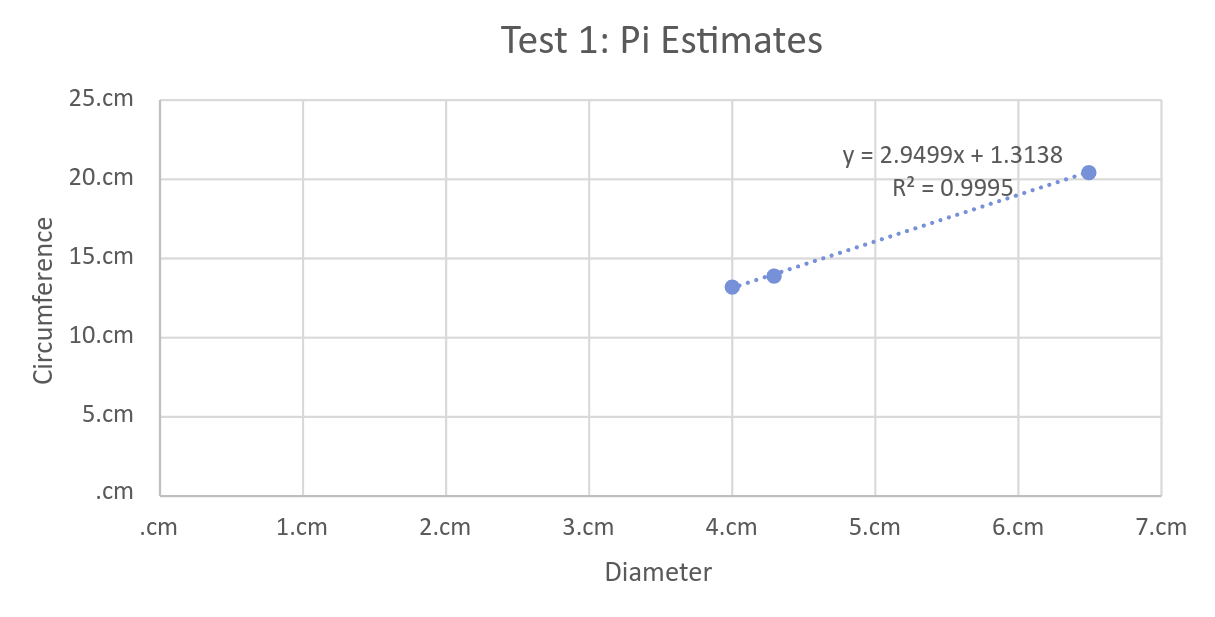
\includegraphics[width=16cm]{lab1_plot1.png}
    \caption{Circumference vs. Diamater of 3 Objects}
    \label{plot:1}
\end{figure}

\setlength{\tabcolsep}{18pt}
\renewcommand{\arraystretch}{1.5}
\begin{table}[H]
\centering
\begin{tabular}{|c|c|c|}
    \hline
    \rowcolor{black}
    \color{white} Object \# & \color{white} Diamater (cm) & \color{white} Circumference (cm) \\
    \hline
    1 & 4.0 cm & 13.2 cm \\
    \hline
    2 & 6.5 cm & 20.5 cm \\
    \hline
    3 & 4.3 cm & 13.9 cm \\
    
    \hline
\end{tabular} 
\caption{Diamater and Circumference of 3 Objects}
\end{table}

\begin{figure}[H]
    \includegraphics*[width=16cm]{lab1_plot3.png}
    \caption{Period of Oscillation vs. Pendulum Length}
    \label{plot:2}
\end{figure}

\begin{table}[H]
\centering
\begin{tabular}{|c|c|}
    \hline
    \rowcolor{black}
    \color{white} Rope Length (cm) & \color{white} Period of Oscillation (s) \\
    \hline
    149.1 cm & 2.46 s \\
    \hline
    129.1 cm & 2.28 s \\
    \hline
    109.1 cm & 1.99 s \\
    \hline
    89.1 cm  & 1.79 s \\
    \hline
    79.1 cm  & 1.61 s \\

    \hline
\end{tabular} 
\caption{Rope Length vs. Period of Oscillation}
\end{table}

\begin{table}[H]
\centering
\begin{tabular}{|c|c|c|}
    \hline
    \rowcolor{black}
    \color{white} Mass (g) & \color{white} Volume ($\mathrm{cm}^3$) & \color{white} Density ($\mathrm{g}/\mathrm{cm}^3$) \\
    \hline
    72.3 g & 122.14 $\mathrm{cm}^3$ & 13.2 $\mathrm{g}/\mathrm{cm}^3$ \\

    \hline
\end{tabular} 
\caption{Mass, Volume, and Density of Wood Block}
\end{table}

\begin{figure}[H]
    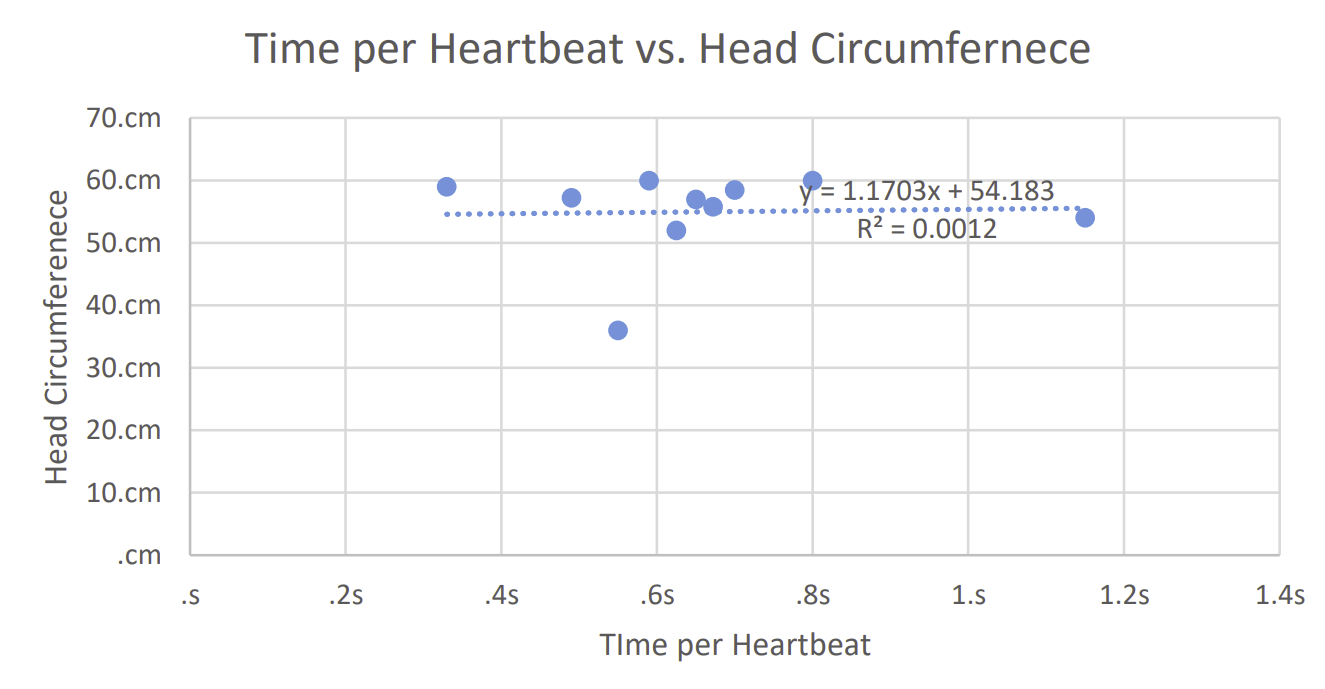
\includegraphics[width=16cm]{lab1_plot2.png}
    \caption{Heart Pulse vs. Head Circumference}
    \label{plot:3}
\end{figure}

\begin{table}[H]
\centering
\begin{tabular}{|c|c|}
    \hline
    \rowcolor{black}
    \color{white} Time Between Heartbeats (s) & \color{white} Head Circumference (cm) \\
    \hline
    0.8 s  & 2.46 cm \\
    \hline
    0.59 s & 2.28 cm \\
    \hline
    0.33 s & 1.99 cm \\
    \hline
    0.7 s  & 1.79 cm \\
    \hline
    0.49 s & 1.61 cm \\
    \hline
    0.65 s & 1.61 cm \\
    \hline
    0.67 s & 1.61 cm \\
    \hline
    1.15 s & 1.61 cm \\
    \hline
    0.63 s & 1.61 cm \\
    \hline
    0.55 s & 1.61 cm \\

    \hline
\end{tabular} 
\caption{Time Between Heartbeats vs. Head Circumference}
\end{table}

\hrule
\vspace{1em}
\section{Questions}
\subsection{Question 1}

\vspace{1em}
\hrule
\vspace{1em}
\section{Conclusion}


\end{document}